%! Date = 6/4/25
\section{Supplementary Motivation}\label{sec:motivation-appx}
\begin{figure}[!ht]
    \centering
    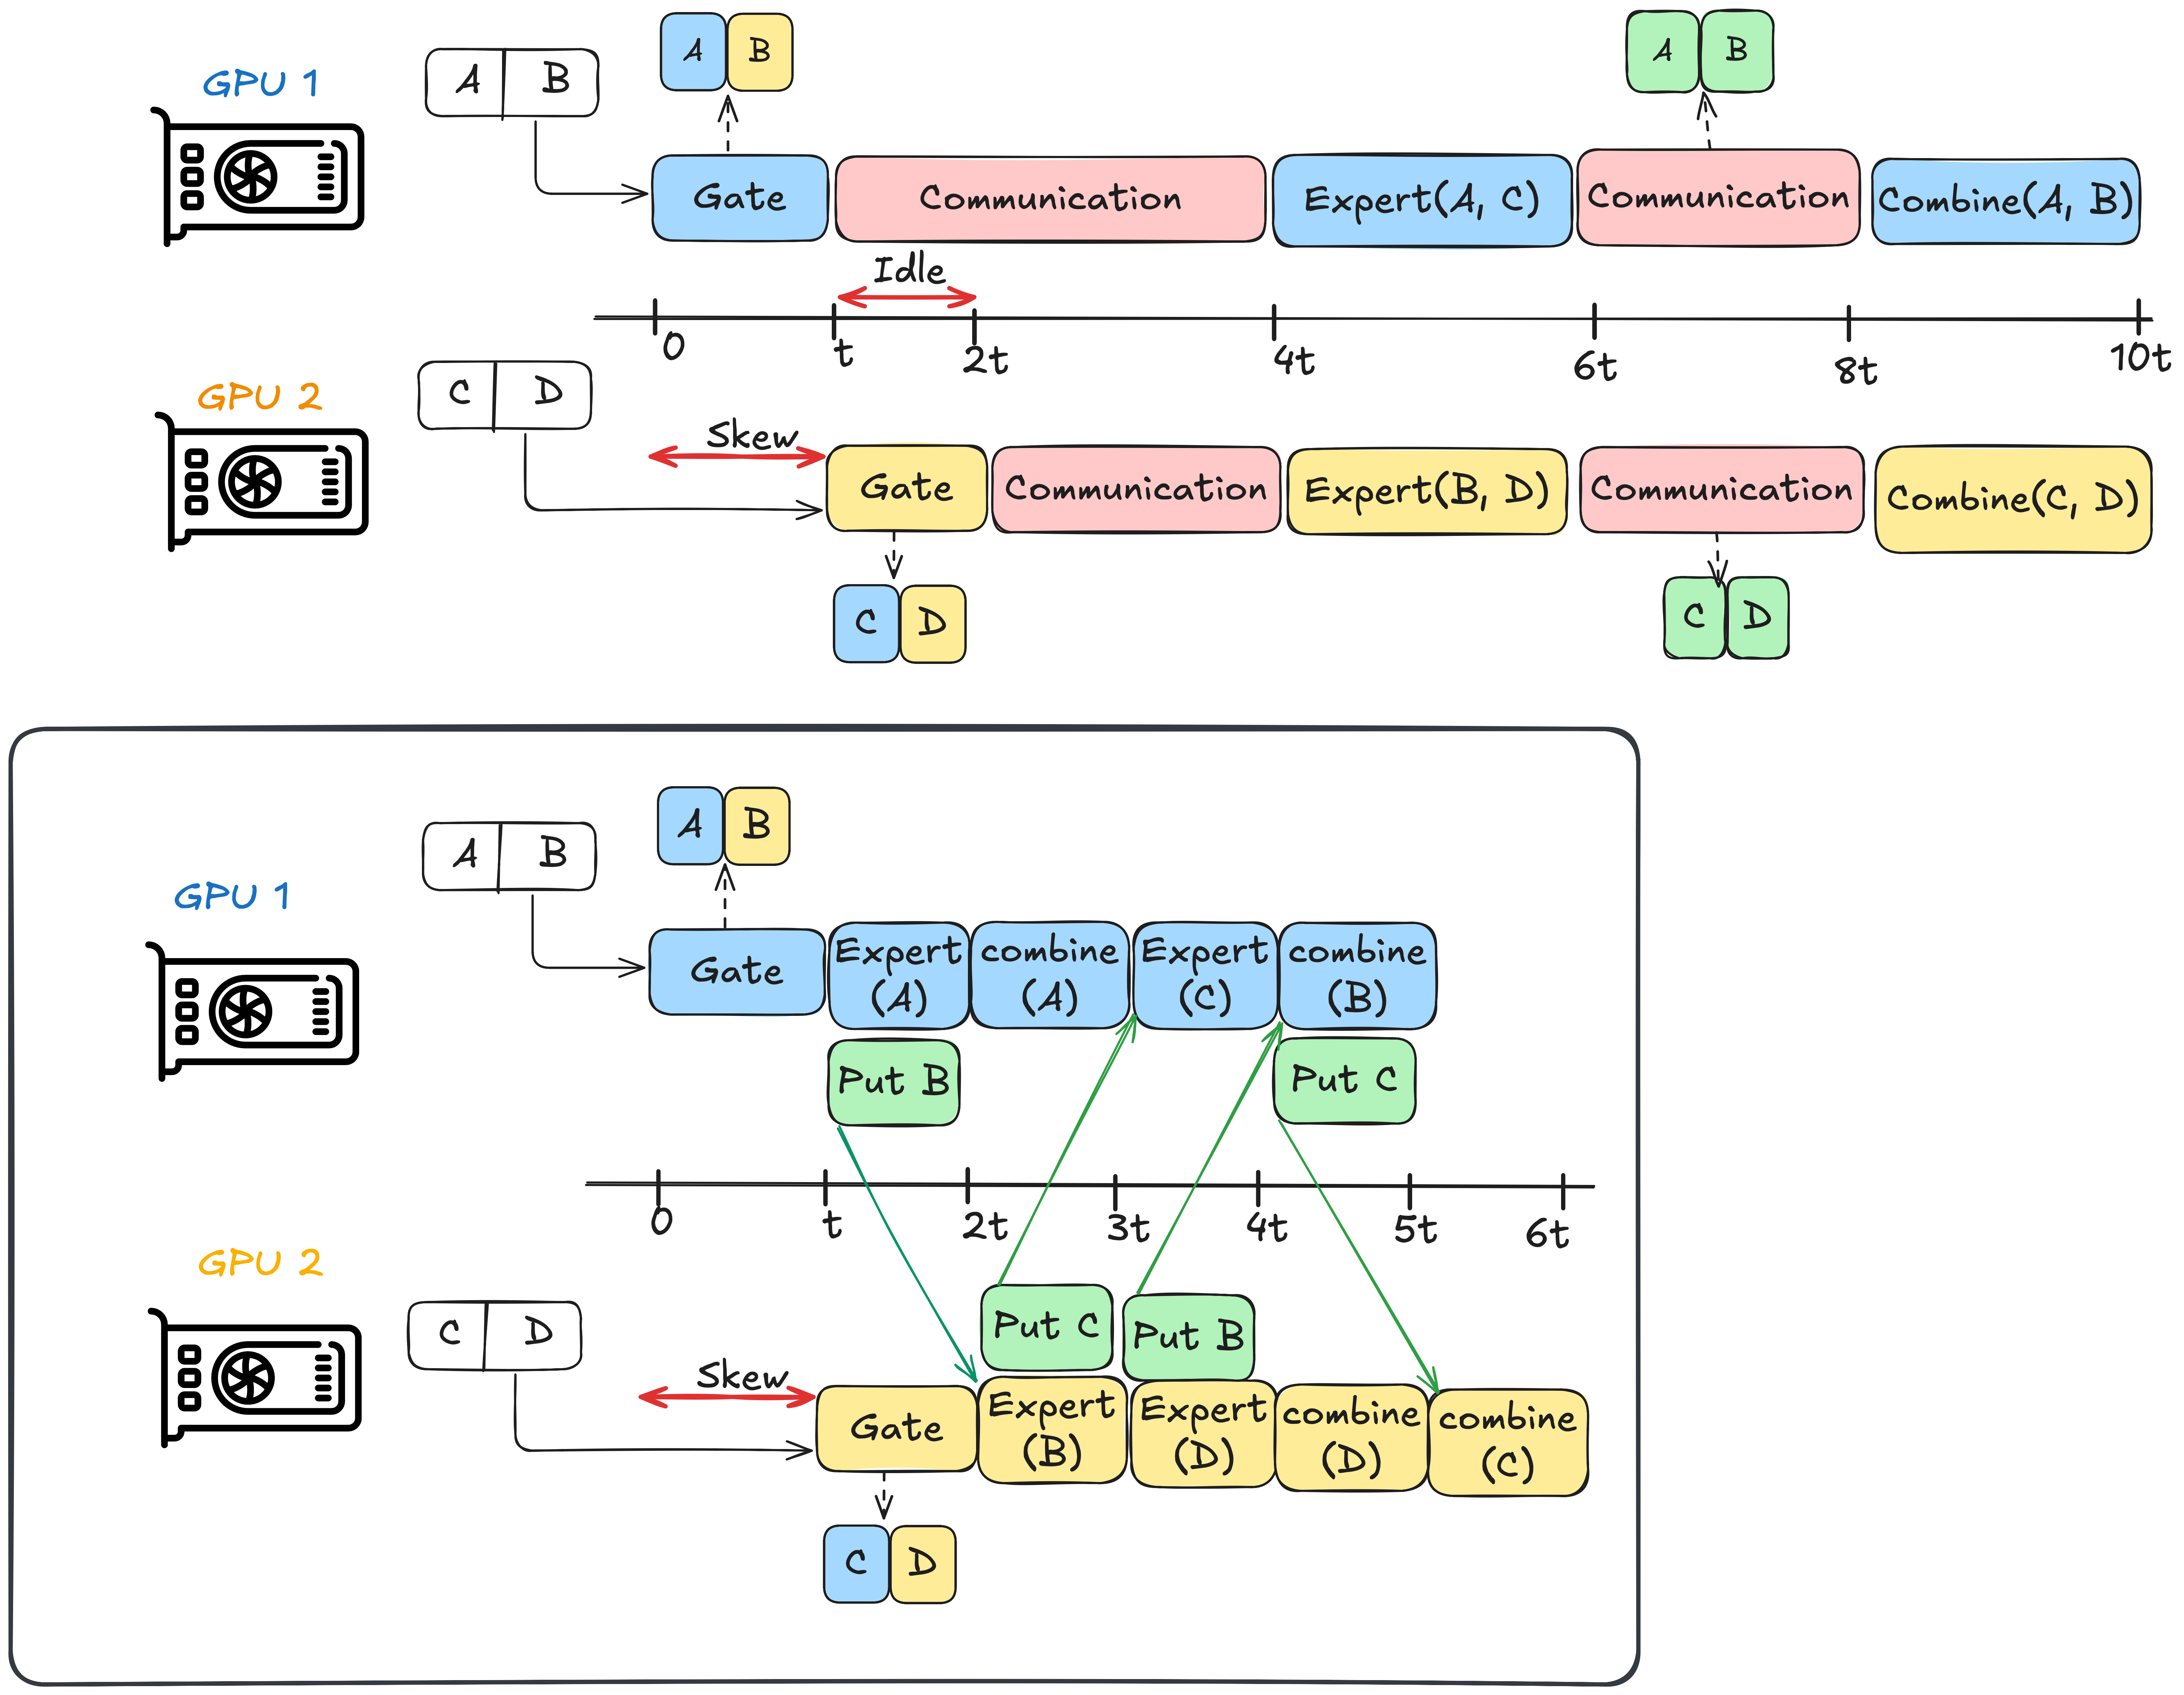
\includegraphics[width=0.8\textwidth, keepaspectratio]{figures/s_overlap}
    \caption{Overlapped Schedule (bottom) showing how idle time from the sequential schedule (top)
        is repurposed for computation. \sysname implements the overlapped schedule.}
    \label{fig:overlap}
\end{figure}
\begin{figure}[!h]
    \centering
    \begin{subfigure}{0.4\textwidth}
        \centering
        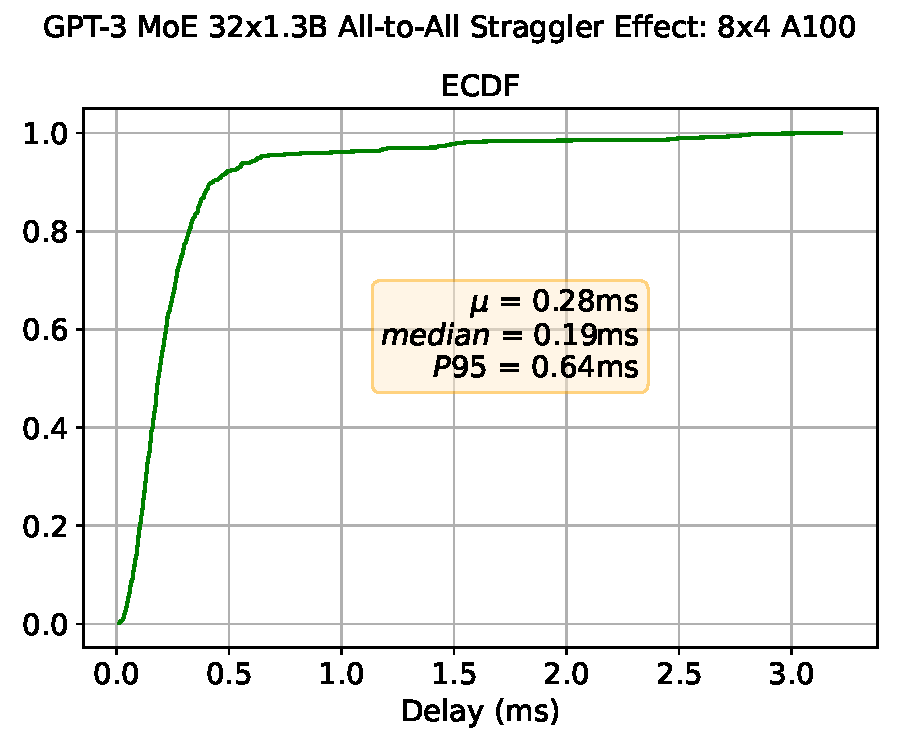
\includegraphics[width=\linewidth, keepaspectratio]{figures/GPT-3_MoE_32x1.3B_ecdf}
        \caption{ECDF}
        \label{sub:ecdf_perl}
    \end{subfigure}
    \begin{subfigure}{0.4\textwidth}
        \centering
        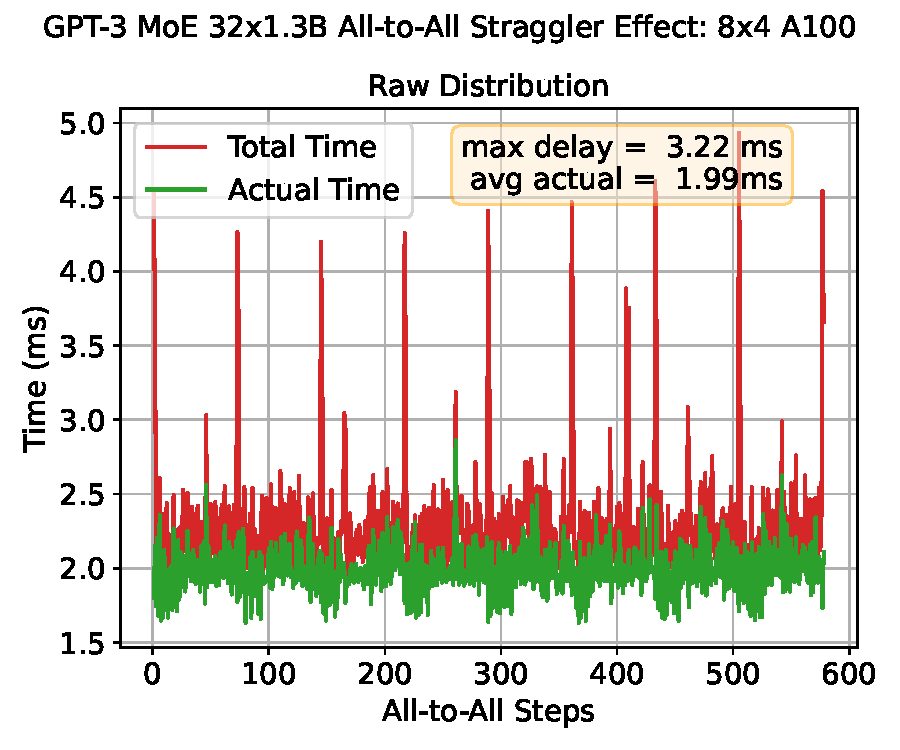
\includegraphics[width=\linewidth, keepaspectratio]{figures/GPT-3_MoE_32x1.3B}
        \caption{Raw Distribution}
        \label{sub:raw_perl}
    \end{subfigure}
    \vspace{1em} % space between rows
    \begin{subfigure}{0.4\textwidth}
        \centering
        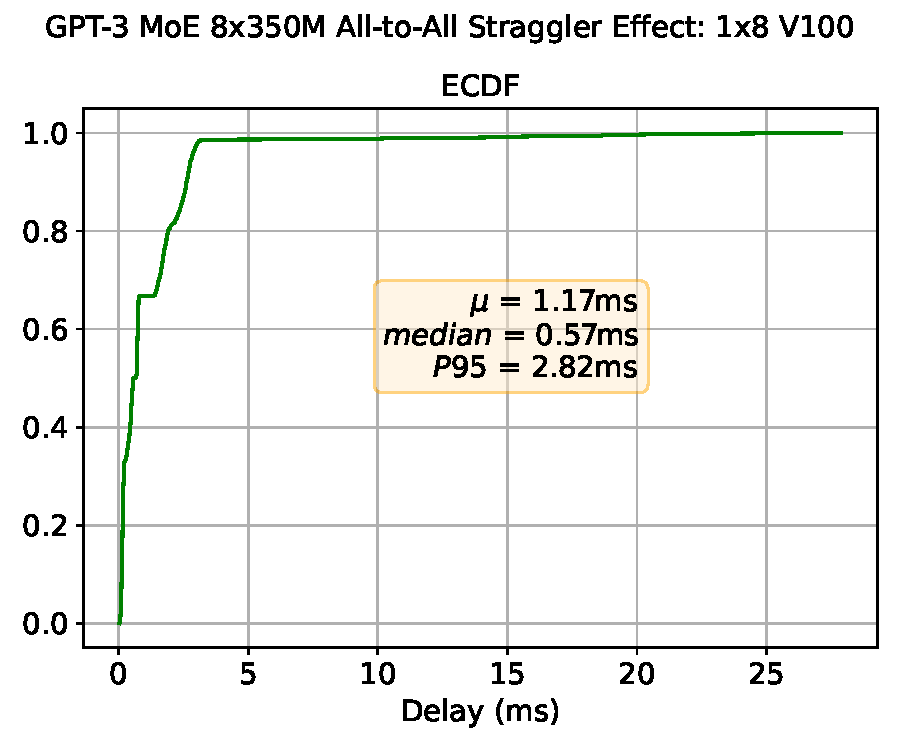
\includegraphics[width=\linewidth, keepaspectratio]{figures/GPT-3_MoE_8x350M_ecdf}
        \caption{ECDF}
        \label{sub:ecdf_az}
    \end{subfigure}
    \begin{subfigure}{0.4\textwidth}
        \centering
        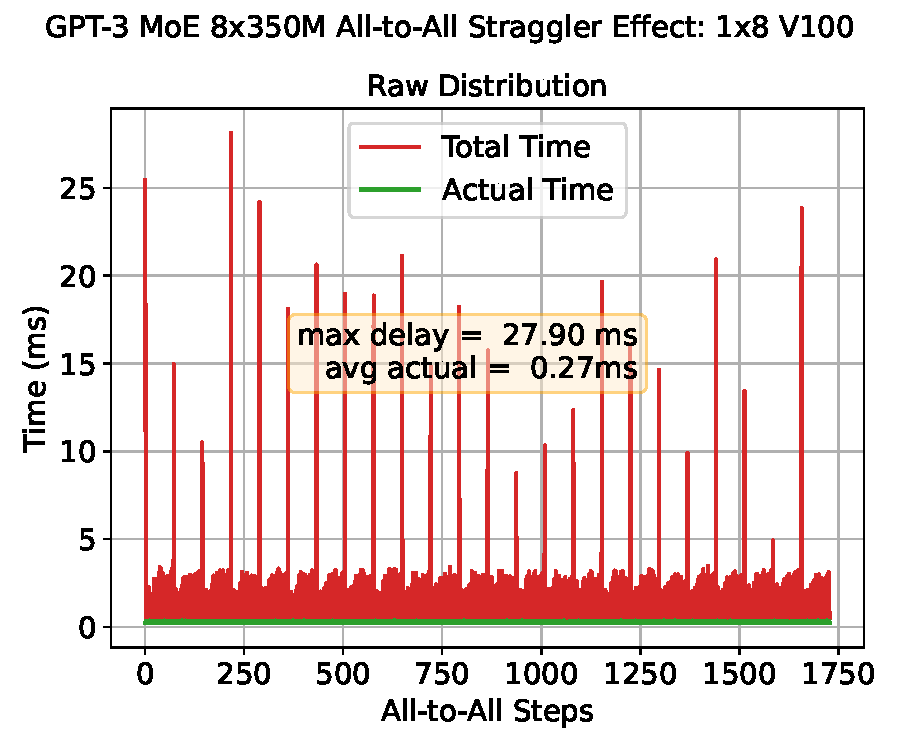
\includegraphics[width=\linewidth, keepaspectratio]{figures/GPT-3_MoE_8x350M}
        \caption{Raw Distribution}
        \label{sub:raw_az}
    \end{subfigure}
    \caption{Straggler effect of synchronous \alltoall. $M\times N$ A100 or V100 denotes
        $N$ GPUs within a node across $M$ nodes.
        Every GPU communicates with every other GPU per~\alltoall step.
        We capture the distribution of delay induced by stragglers across many steps.
        \textbf{Actual Time} $t_a$ denotes the fastest kernel execution time across all GPUs,
        conversely \textbf{Total Time} $t$ is the maximum recorded step time, while
        $Delay$ is the maximum difference between $t$ and $t_a$. Note $Delay$ is idle time.}
    \label{fig:straggler}
\end{figure}
Specifically, as shown in Figure~\ref{fig:straggler}, for distributed training of a 1.3B GPT-3 MoE model across
32 A100 GPUs, we see P95 communication performance degradation of \textbf{1.32X} when compared to the mean actual kernel time
from Figure~\ref{sub:raw_perl}.
This performance reduction is rather tame as the underlying hardware is a supercomputer well-tuned
against ``software jitter''~\cite{nerscNetworkNERSC}.
However, we observe a more severe p95 performance loss of \textbf{11X} in a single-node Virtual Machine (VM).
In line with prior HPC works~\cite{1639320, 10.1145/3545008.3545056},
we argue that obviating the inherent barrier in this synchronous collective communication would
allow GPUs to repurpose this observed idle time for downstream computation as depicted in Figure~\ref{fig:overlap}.
\begin{table}[!h]
    \centering
    \caption{Straggler Delay within Synchronous \emph{All-to-All} communication.
    We capture the distribution of delay induced by stragglers across many steps.
    Let \textbf{Actual Time} $t_a$ denote the fastest kernel execution time across all GPUs,
        and \textbf{Total Time} $t$ be the maximum recorded step time. We define
        $Delay$ as the maximum difference between $t$ and $t_a$. Note $Delay$ is idle time. For the
        1x8 V100, we profile 1750 steps and 600 steps for the 8x4 A100. See Figure~\ref{fig:straggler}
        for the raw distribution.}
    \label{tab:s_delays}
    \begin{tabular}{@{}lcccc@{}}
        \toprule
        \textbf{System}      & \multicolumn{1}{l}{\textbf{\# Nodes}} & \multicolumn{1}{l}{\textbf{\# GPUs}} & \textbf{Median} & \textbf{p95} \\ \midrule
        Commercial VM (V100) & 1                                     & 8                                    & 3.1x            & 11.4x        \\
        Supercomputer (A100) & 8                                     & 32                                   & 1.09x           & 1.32x        \\ \bottomrule
    \end{tabular}
\end{table}
